\chapter{Υλοποίηση}

Έχοντας κατανοήσει τη θεωρία της γραφικής υπολογιστών και της υπολογιστικής γεωμετρίας αναφορικά με την χάραξη πολυγώνων, είμαστε σε θέση να ερμηνεύσουμε τον δοθέντα αλγόριθμο χάραξης τριγώνου και να τον γενικεύσουμε σε έναν αλγόριθμο χάραξης κυρτών πολυγώνων.

\section{Επεξήγηση διαδικασίας \textlatin{triangle1}}
H διαδικασία \textlatin{triangle1} περιγράφει έναν απλό αλγόριθμο ψηφιδόξυσης τριγώνου. Η συνάρτηση δέχεται ως ορίσματα τις τρεις κορυφές του τριγώνου και την τιμή χρωματισμού των εικονοστοιχείων ευρισκόμενων εντός του πολυγώνου. Αφού αρχικοποιήσουμε τις μεταβλητές των ακμών και των γραμμικών συναρτήσεων, καλούμε την κατάλληλη συνάρτηση για να σχεδιάσουμε τις ακμές του τριγώνου. Ακολουθεί ο υπολογισμός του περιβάλλοντος κυτίου του τριγώνου, η εκτίμηση των γραμμικών συναρτήσεων στο κατώτερο σημείο του, και η αποθήκευσή τους στις αντίστοιχες προσωρινές μεταβλητές, με σκοπό τον έλεγχο των προσήμων των συναρτήσεων και κατ’ επέκταση τον προσδιορισμό της θέσης κάθε εικονοστοιχείου. Για κάθε εικονοστοιχείο $p$ του περιβάλλοντος κυτίου, εάν οι τιμές και των τριών συναρτήσεων έχουν το ίδιο πρόσημο, τότε το $p$ ευρίσκεται εντός του τριγώνου, αλλιώς ευρίσκεται εκτός αυτού (Δρακόπουλος, 2021, σ. 152? Σπύρου, 2019, σ. 60). Για ομόσημες γραμμικές συναρτήσεις, καλούμε τη συνάρτηση χρωματισμού εικονοστοιχείου και, μέσω του διπλού βρόχου επανάληψης, επιτυγχάνεται τελικώς η ψηφιδόξυση του τριγώνου.

\section{Γενίκευση διαδικασίας \textlatin{triangle1} στην \textlatin{convex1}}
Εφόσον κάθε πολύγωνο δύναται να κατασκευαστεί από τρίγωνα, η διαδικασία χάραξης τριγώνων \textlatin{triangle1} δύναται να γενικευθεί παρομοίως στη διαδικασία χάραξης κυρτών πολυγώνων \textlatin{convex1}. Αρχικά, η συνάρτηση \textlatin{convex1} δέχεται ως ορίσματα την τιμή χρωματισμού των εικονοστοιχείων ευρισκόμενων εντός του πολυγώνου, και ένα πλήθος σημείων $S$ ορισμένο από τον χρήστη. Κατόπιν, αρχικοποιούνται οι απαραίτητες μεταβλητές για τον έλεγχο κυρτότητας, τον σχεδιασμό ακμών και τον υπολογισμό των γραμμικών συναρτήσεων του πολυγώνου. \par

Η επιλογή του αλγορίθμου περιτυλίγματος για τον έλεγχο κυρτότητας του πολυγώνου βασίζεται στην προμελετηθείσα θεωρία. Ο αλγόριθμος υλοποιείται καλώντας τη συνάρτηση \textlatin{jarvis} με όρισμα το μέγεθος του πίνακα σημείων στο επίπεδο, δηλαδή το σύνολο των δυνητικών κορυφών του πολυγώνου. Αρχικά, αποθηκεύουμε την τιμή του αριστερότερου σημείου του συνόλου στη μεταβλητή $leftPoint$, και υλοποιούμε τον διπλό βρόχο επανάληψης του αλγορίθμου περιτυλίγματος. Συγκεκριμένα, ορίζουμε το $p[i]$ ως το αριστερότερο σημείο του επιπέδου, και επιλέγουμε αυθαίρετα ως τελικό σημείο $endPoint$ το πρώτο σημείο του συνόλου $S$. Στον εσωτερικό βρόχο ελέγχουμε εάν το τελικό σημείο και το αριστερότερο σημείο ταυτίζονται, ή εάν το τρέχον σημείο που εξετάζεται είναι αριστερότερα του $leftPoint$. Αν ισχύει οιαδήποτε εκ των δύο συνθηκών, θέτουμε το τελικό σημείο ίσο με το τρέχον σημείο και καλούμε την κατάλληλη συνάρτηση για τη σχεδίαση των ακμών, ενώ στον εξωτερικό βρόχο αποθηκεύουμε την τιμή του τελικού σημείου στη θέση του αριστερότερου σημείου. Οι επαναλήψεις τερματίζουν όταν το τελικό σημείο ταυτιστεί με το πρώτο σημείο του πολυγώνου, δηλαδή όταν η πολυγωνική αλυσίδα των κορυφών κλείσει και σχηματίσει το κυρτό περίβλημα (Κωστόπουλος, 2013? \textlatin{Jarvis, 1973; Sharma, 2018}). \par

\begin{figure}[h]
\centering
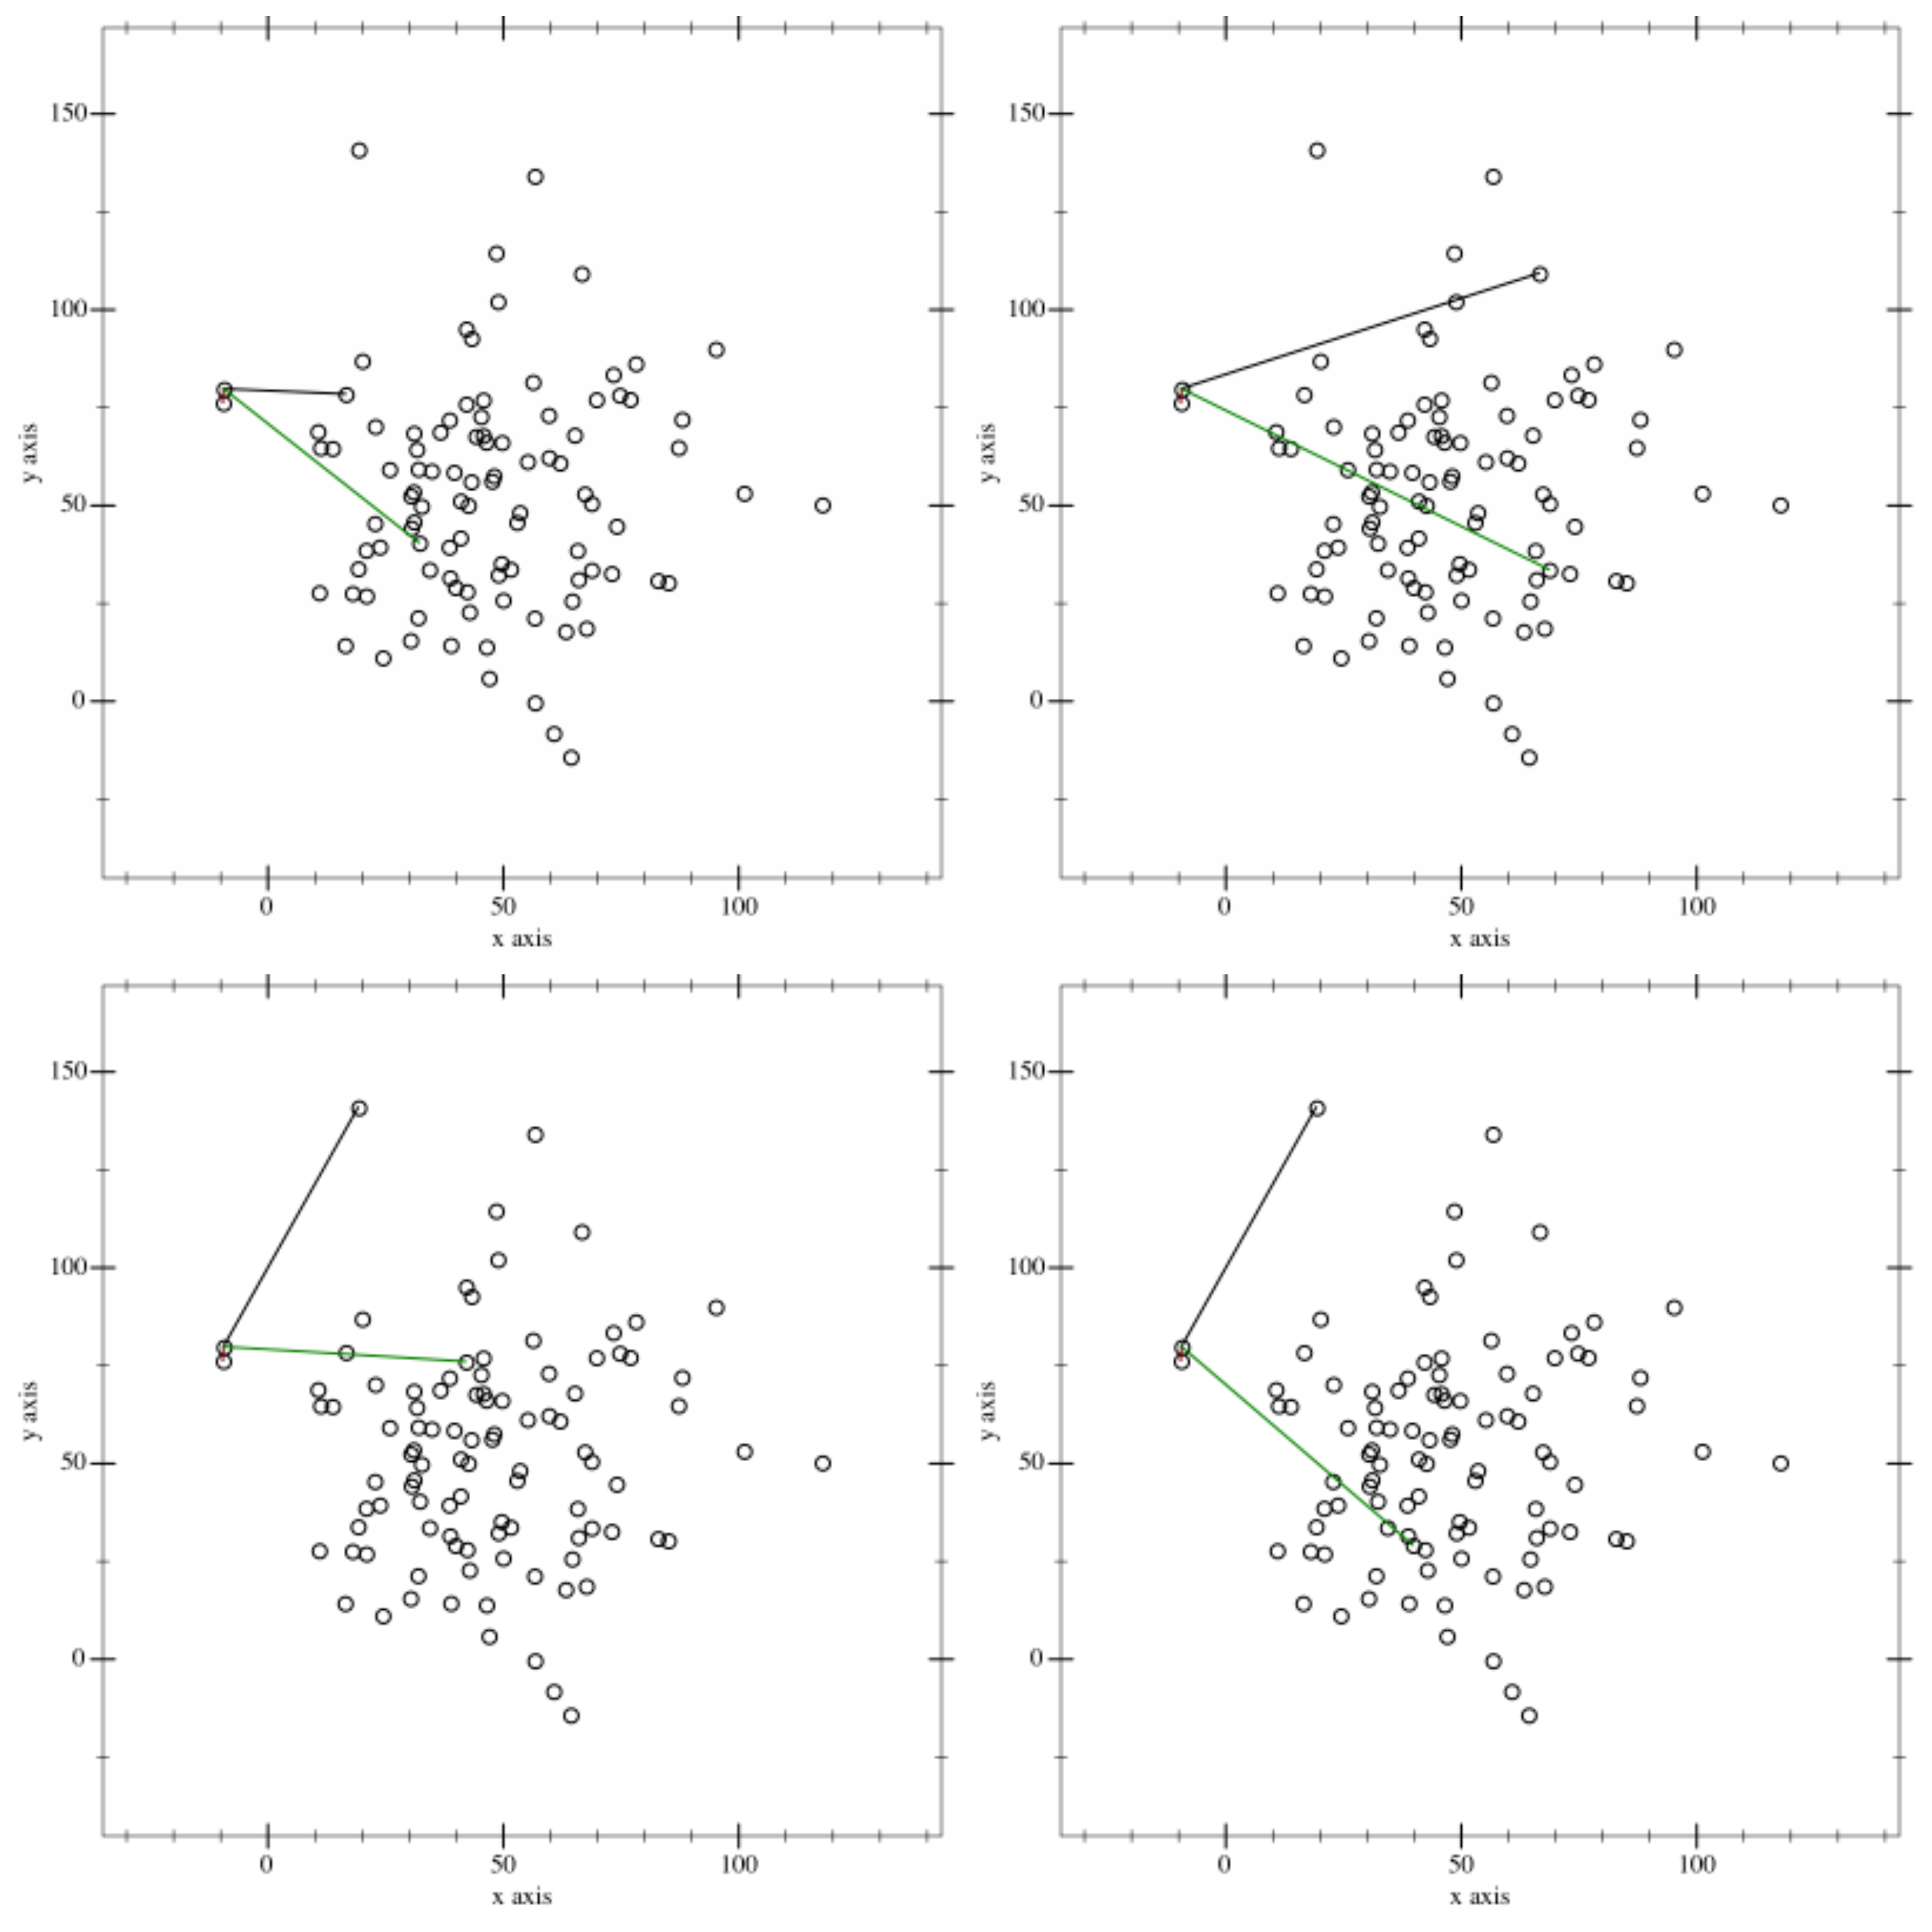
\includegraphics[width=0.45\textwidth]{images/jarvis}
\caption{Στιγμιότυπα εκτέλεσης του αλγορίθμου περιτυλίγματος (\textlatin{Sharma}, 2018)}
\end{figure}

Η υπόλοιπη διαδικασία\footnote{Υπολογισμός του περιβάλλοντος κυτίου του πολυγώνου, εκτίμηση των γραμμικών συναρτήσεων στο σημείο $bb\_xmin, bb\_ymin$, έλεγχος προσήμων των γραμμικών συναρτήσεων} \textlatin{convex1} ακολουθεί τα βήματα της \textlatin{triangle1}, χρησιμοποιώντας πίνακες αποθήκευσης των κορυφών, των ακμών και των γραμμικών συναρτήσεων, και καλώντας βρόχους επανάληψης για την υλοποίηση των πράξεων, δεδομένου ότι δεν αφορά γνωστό πλήθος κορυφών, αλλά αυθαίρετα παραγόμενο σύνολο σημείων στο επίπεδο. \par

\subsection{Υλοποίηση σε \textlatin{OpenGL}}

Tμήμα της υλοποίησης εκφράστηκε στη γλώσσα προγραμματισμού \textlatin{C++} με τη βοήθεια της \textlatin{OpenGL}. Η \textlatin{OpenGL} αποτελεί πρότυπο καθορισμού λειτουργιών που πρέπει να υποστηρίζει μια βιβλιοθήκη γραφικών για να είναι συμβατή με αυτήν. Είναι ανεξάρτητη λειτουργικού συστήματος και ορίζει µια προγραµµατιστική διεπιφάνεια σχεδίασης γραφικών (Δρακόπουλος, 2022). \par

Ο εκτελέσιμος κώδικας περιέχει συναρτήσεις \textbf{\textlatin{void}} για τη χάραξη κυρτού πολυγώνου και τη δημιουργία σχήματος με την χρήση του ποντικιού. Αναλυτικότερα, στο πεδίο της \textbf{\textlatin{void mouse}} ορίζεται η κλήση του ποντικιού για το τρέχον παράθυρο και με κάθε πάτημα-απελευθέρωσή του, αποστέλλονται σήματα που υποδεικνύουν τις συντεταγμένες $x$ και $y$ των κορυφών του πολυγώνου. Κατά την \textbf{\textlatin{void display}} ορίζεται το χρώμα σχεδίασης και η δημιουργία του πολυγώνου βάσει των εντολών που αναγράφονται στον παρακάτω πίνακα, καθώς και στο αρχείο του κώδικα. Τελικώς, οι παραπάνω συναρτήσεις καλούνται στην \textbf{\textlatin{main}} συνάρτηση του προγράμματος για την ψηφιδόξυση πολυγώνων με κορυφές ορισμένες από την αλληλεπίδραση του χρήστη με το παράθυρο εφαρμογής. \par

\vspace{2em}

\begin{center}
    \begin{longtable}{p{6.5cm}|p{7cm}} 
        \textbf{Εντολές} & \textbf{Εξήγηση} \\ \hline \hline
        \textlatin{\lstinline[language=C]!void mouse()!} & Συνάρτηση διαχείρισης σημάτων από το ποντίκι \\ \hline
        \textlatin{\lstinline[language=C]!GLUT_LEFT_BUTTON / GLUT_UP!} & Λήψη σήματος κατά την απελευθέρωση του αριστερού κουμπιού του ποντικιού \\ \hline
        \textlatin{\lstinline[language=C]!void display()!} & Συνάρτηση που διαχειρίζεται τι σχεδιάζεται στην οθόνη και με ποια σειρά \\ \hline
        \textlatin{\lstinline[language=C]!glColor3f(1, 0, 0)!} & Επιλογή χρώµατος σχεδίασης (κόκκινο) \\ \hline
        \textlatin{\lstinline[language=C]!glMatrixMode(GL_PROJECTION)!}  & Επιλογή μητρώου προβολής \\ \hline
        \textlatin{\lstinline[language=C]!glLoadIdentity!} & Αντικατάσταση τρέχοντος μητρώου από το μητρώο προβολής \\ \hline
        \textlatin{\lstinline[language=C]!gluOrtho2D(0, 640, 0, 480)!} & Δήλωση παράλληλης προβολής \\
        \hline
        \textlatin{\lstinline[language=C]!glBegin(GL_POLYGON) / glEnd!} & Μεταξύ αυτών των εντολών δηλώνονται συντεταγµένες κορυφών κυρτού πολυγώνου \\ \hline
        \textlatin{\lstinline[language=C]!glVertex2f(x, y)!} & Δήλωση συντεταγµένων μεμονομένων κορυφών (δύο παράμετροι τύπου \textlatin{float}) \\ \hline
        \textlatin{\lstinline[language=C]!glFlush!} & Προώθηση εκτέλεσης εκκρεμούντων εντολών \\ \hline
        \textlatin{\lstinline[language=C]!glutInitWindowSize(640, 480)!} & Ορισμός διαστάσεων παραθύρου εφαρµογής σε \textlatin{pixels} \\ \hline
        \textlatin{\lstinline[language=C]!glutInitWindowPosition(100, 100)!} & Δήλωση θέσης παραθύρου εφαρμογής στην οθόνη \\ \hline
        \textlatin{\lstinline[language=C]!glutInitDisplayMode!} & Καθορίζει ρυθµίσεις απεικόνισης (µοντέλο ενταµίευσης, χρωµατικό µοντέλο κ.λ.π.) \\ \hline
        \textlatin{\lstinline[language=C]!GLUT_SINGLE | GLUT_RGB!} & Δήλωση μοντέλου απλής ενταμίευσης (\textlatin{single buffer}) και χρωματικού μοντέλου \textlatin{RGB} \\ \hline
        \textlatin{\lstinline[language=C]!glutCreateWindow("Convex1")!} & Εµφάνιση παραθύρου εφαρµογής \\ \hline
        \textlatin{\lstinline[language=C]!glClearColor(1,1,1,0)!} & Δήλωση χρώµατος καθαρισµού της οθόνης (λευκό) \\ \hline
        \textlatin{\lstinline[language=C]!glClear!} & Καθαρισµός ενός από τους ενταµιευτές του συστήµατος γραφικών \\ \hline
        \textlatin{\lstinline[language=C]!glutDisplayFunc(display)!} & Κλήση συνάρτησης σχεδιασμού της σκηνής \\ \hline
        \textlatin{\lstinline[language=C]!glutMouseFunc(mouse)!} & Κλήση συνάρτησης αλληλεπίδρασης με το ποντίκι \\ \hline
        \textlatin{\lstinline[language=C]!glutMainLoop()!} & Ενεργοποίηση κύκλου ακρόασης γεγονότων \\ \hline
    \caption{Πίναξ εντολών \textlatin{OpenGL}}
    \end{longtable}
\end{center}
